% REV01 Tue 22 Jun 2021 12:46:10 WIB
% START Tue 04 May 2021 13:55:16 WIB

\chapter{LODGERS IN QUEER STREET}

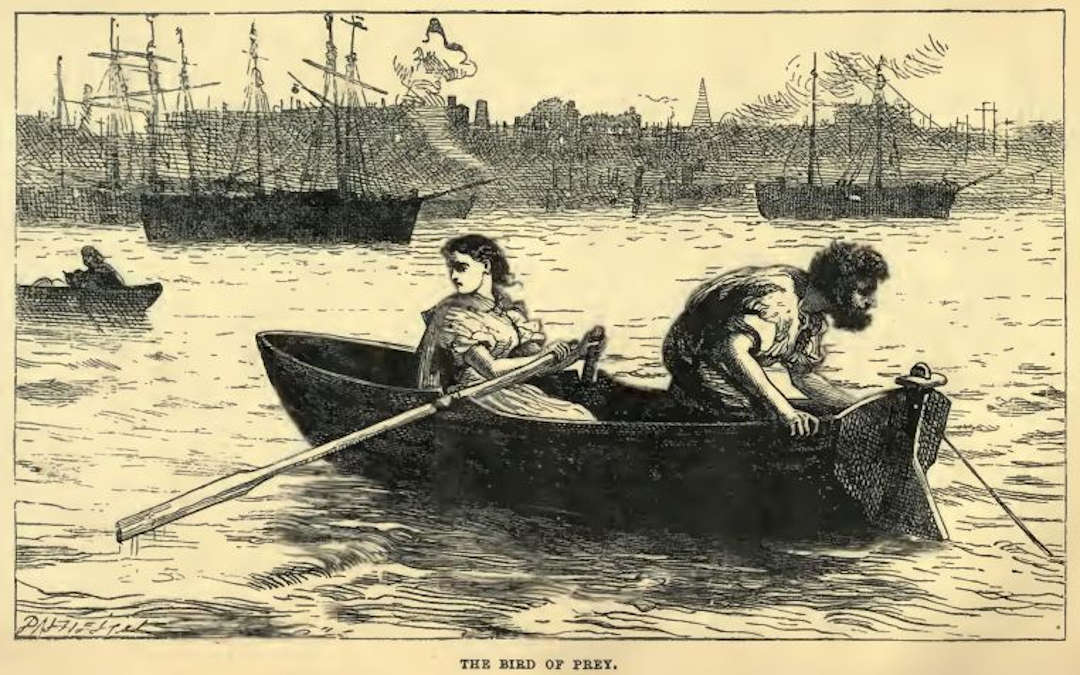
\includegraphics[scale=2.3]{01-01-01}

It was a foggy day in London, and the fog was heavy and dark. Animate
London, with smarting eyes and irritated lungs, was blinking, wheezing,
and choking; inanimate London was a sooty spectre, divided in purpose
between being visible and invisible, and so being wholly neither.
Gaslights flared in the shops with a haggard and unblest air, as knowing
themselves to be night-creatures that had no business abroad under the
sun; while the sun itself when it was for a few moments dimly indicated
through circling eddies of fog, showed as if it had gone out and were
collapsing flat and cold. Even in the surrounding country it was a foggy
day, but there the fog was grey, whereas in London it was, at about
the boundary line, dark yellow, and a little within it brown, and then
browner, and then browner, until at the heart of the City--which call
Saint Mary Axe--it was rusty-black. From any point of the high ridge of
land northward, it might have been discerned that the loftiest buildings
made an occasional struggle to get their heads above the foggy sea, and
especially that the great dome of Saint Paul’s seemed to die hard; but
this was not perceivable in the streets at their feet, where the whole
metropolis was a heap of vapour charged with muffled sound of wheels,
and enfolding a gigantic catarrh.

At nine o’clock on such a morning, the place of business of Pubsey and
Co. was not the liveliest object even in Saint Mary Axe--which is not a
very lively spot--with a sobbing gaslight in the counting-house window,
and a burglarious stream of fog creeping in to strangle it through the
keyhole of the main door. But the light went out, and the main door
opened, and Riah came forth with a bag under his arm.

Almost in the act of coming out at the door, Riah went into the fog, and
was lost to the eyes of Saint Mary Axe. But the eyes of this history
can follow him westward, by Cornhill, Cheapside, Fleet Street, and the
Strand, to Piccadilly and the Albany. Thither he went at his grave and
measured pace, staff in hand, skirt at heel; and more than one head,
turning to look back at his venerable figure already lost in the mist,
supposed it to be some ordinary figure indistinctly seen, which fancy
and the fog had worked into that passing likeness.

Arrived at the house in which his master’s chambers were on the
second floor, Riah proceeded up the stairs, and paused at Fascination
Fledgeby’s door. Making free with neither bell nor knocker, he struck
upon the door with the top of his staff, and, having listened, sat down
on the threshold. It was characteristic of his habitual submission,
that he sat down on the raw dark staircase, as many of his ancestors
had probably sat down in dungeons, taking what befell him as it might
befall.

After a time, when he had grown so cold as to be fain to blow upon his
fingers, he arose and knocked with his staff again, and listened again,
and again sat down to wait. Thrice he repeated these actions before his
listening ears were greeted by the voice of Fledgeby, calling from his
bed, ‘Hold your row!--I’ll come and open the door directly!’ But, in
lieu of coming directly, he fell into a sweet sleep for some quarter of
an hour more, during which added interval Riah sat upon the stairs and
waited with perfect patience.

At length the door stood open, and Mr Fledgeby’s retreating drapery
plunged into bed again. Following it at a respectful distance, Riah
passed into the bed-chamber, where a fire had been sometime lighted, and
was burning briskly.

‘Why, what time of night do you mean to call it?’ inquired Fledgeby,
turning away beneath the clothes, and presenting a comfortable rampart
of shoulder to the chilled figure of the old man.

‘Sir, it is full half-past ten in the morning.’

‘The deuce it is! Then it must be precious foggy?’

‘Very foggy, sir.’

‘And raw, then?’

‘Chill and bitter,’ said Riah, drawing out a handkerchief, and wiping
the moisture from his beard and long grey hair as he stood on the verge
of the rug, with his eyes on the acceptable fire.

With a plunge of enjoyment, Fledgeby settled himself afresh.

‘Any snow, or sleet, or slush, or anything of that sort?’ he asked.

‘No, sir, no. Not quite so bad as that. The streets are pretty clean.’

‘You needn’t brag about it,’ returned Fledgeby, disappointed in his
desire to heighten the contrast between his bed and the streets. ‘But
you’re always bragging about something. Got the books there?’

‘They are here, sir.’

‘All right. I’ll turn the general subject over in my mind for a minute
or two, and while I’m about it you can empty your bag and get ready for
me.’

With another comfortable plunge, Mr Fledgeby fell asleep again. The old
man, having obeyed his directions, sat down on the edge of a chair, and,
folding his hands before him, gradually yielded to the influence of the
warmth, and dozed. He was roused by Mr Fledgeby’s appearing erect at
the foot of the bed, in Turkish slippers, rose-coloured Turkish trousers
(got cheap from somebody who had cheated some other somebody out of
them), and a gown and cap to correspond. In that costume he would have
left nothing to be desired, if he had been further fitted out with a
bottomless chair, a lantern, and a bunch of matches.

‘Now, old ‘un!’ cried Fascination, in his light raillery, ‘what dodgery
are you up to next, sitting there with your eyes shut? You ain’t asleep.
Catch a weasel at it, and catch a Jew!’

‘Truly, sir, I fear I nodded,’ said the old man.

‘Not you!’ returned Fledgeby, with a cunning look. ‘A telling move with
a good many, I dare say, but it won’t put ME off my guard. Not a bad
notion though, if you want to look indifferent in driving a bargain. Oh,
you are a dodger!’

The old man shook his head, gently repudiating the imputation, and
suppressed a sigh, and moved to the table at which Mr Fledgeby was now
pouring out for himself a cup of steaming and fragrant coffee from a pot
that had stood ready on the hob. It was an edifying spectacle, the young
man in his easy chair taking his coffee, and the old man with his grey
head bent, standing awaiting his pleasure.

‘Now!’ said Fledgeby. ‘Fork out your balance in hand, and prove by
figures how you make it out that it ain’t more. First of all, light that
candle.’

Riah obeyed, and then taking a bag from his breast, and referring to
the sum in the accounts for which they made him responsible, told it out
upon the table. Fledgeby told it again with great care, and rang every
sovereign.

‘I suppose,’ he said, taking one up to eye it closely, ‘you haven’t been
lightening any of these; but it’s a trade of your people’s, you know.
YOU understand what sweating a pound means, don’t you?’

‘Much as you do, sir,’ returned the old man, with his hands under
opposite cuffs of his loose sleeves, as he stood at the table,
deferentially observant of the master’s face. ‘May I take the liberty to
say something?’

‘You may,’ Fledgeby graciously conceded.

‘Do you not, sir--without intending it--of a surety without intending
it--sometimes mingle the character I fairly earn in your employment,
with the character which it is your policy that I should bear?’

‘I don’t find it worth my while to cut things so fine as to go into the
inquiry,’ Fascination coolly answered.

‘Not in justice?’

‘Bother justice!’ said Fledgeby.

‘Not in generosity?’

‘Jews and generosity!’ said Fledgeby. ‘That’s a good connexion! Bring
out your vouchers, and don’t talk Jerusalem palaver.’

The vouchers were produced, and for the next half-hour Mr Fledgeby
concentrated his sublime attention on them. They and the accounts were
all found correct, and the books and the papers resumed their places in
the bag.

‘Next,’ said Fledgeby, ‘concerning that bill-broking branch of the
business; the branch I like best. What queer bills are to be bought, and
at what prices? You have got your list of what’s in the market?’

‘Sir, a long list,’ replied Riah, taking out a pocket-book, and
selecting from its contents a folded paper, which, being unfolded,
became a sheet of foolscap covered with close writing.

‘Whew!’ whistled Fledgeby, as he took it in his hand. ‘Queer Street is
full of lodgers just at present! These are to be disposed of in parcels;
are they?’

‘In parcels as set forth,’ returned the old man, looking over his
master’s shoulder; ‘or the lump.’

‘Half the lump will be waste-paper, one knows beforehand,’ said
Fledgeby. ‘Can you get it at waste-paper price? That’s the question.’

Riah shook his head, and Fledgeby cast his small eyes down the list.
They presently began to twinkle, and he no sooner became conscious of
their twinkling, than he looked up over his shoulder at the grave face
above him, and moved to the chimney-piece. Making a desk of it, he stood
there with his back to the old man, warming his knees, perusing the list
at his leisure, and often returning to some lines of it, as though
they were particularly interesting. At those times he glanced in the
chimney-glass to see what note the old man took of him. He took none
that could be detected, but, aware of his employer’s suspicions, stood
with his eyes on the ground.

Mr Fledgeby was thus amiably engaged when a step was heard at the outer
door, and the door was heard to open hastily. ‘Hark! That’s your doing,
you Pump of Israel,’ said Fledgeby; ‘you can’t have shut it.’ Then the
step was heard within, and the voice of Mr Alfred Lammle called aloud,
‘Are you anywhere here, Fledgeby?’ To which Fledgeby, after cautioning
Riah in a low voice to take his cue as it should be given him, replied,
‘Here I am!’ and opened his bedroom door.

‘Come in!’ said Fledgeby. ‘This gentleman is only Pubsey and Co. of
Saint Mary Axe, that I am trying to make terms for an unfortunate friend
with in a matter of some dishonoured bills. But really Pubsey and Co.
are so strict with their debtors, and so hard to move, that I seem to be
wasting my time. Can’t I make ANY terms with you on my friend’s part, Mr
Riah?’

‘I am but the representative of another, sir,’ returned the Jew in a low
voice. ‘I do as I am bidden by my principal. It is not my capital that
is invested in the business. It is not my profit that arises therefrom.’

‘Ha ha!’ laughed Fledgeby. ‘Lammle?’

‘Ha ha!’ laughed Lammle. ‘Yes. Of course. We know.’

‘Devilish good, ain’t it, Lammle?’ said Fledgeby, unspeakably amused by
his hidden joke.

‘Always the same, always the same!’ said Lammle. ‘Mr--’

‘Riah, Pubsey and Co. Saint Mary Axe,’ Fledgeby put in, as he wiped away
the tears that trickled from his eyes, so rare was his enjoyment of his
secret joke.

‘Mr Riah is bound to observe the invariable forms for such cases made
and provided,’ said Lammle.

‘He is only the representative of another!’ cried Fledgeby. ‘Does as
he is told by his principal! Not his capital that’s invested in the
business. Oh, that’s good! Ha ha ha ha!’ Mr Lammle joined in the laugh
and looked knowing; and the more he did both, the more exquisite the
secret joke became for Mr Fledgeby.

‘However,’ said that fascinating gentleman, wiping his eyes again, ‘if
we go on in this way, we shall seem to be almost making game of Mr Riah,
or of Pubsey and Co. Saint Mary Axe, or of somebody: which is far from
our intention. Mr Riah, if you would have the kindness to step into the
next room for a few moments while I speak with Mr Lammle here, I should
like to try to make terms with you once again before you go.’

The old man, who had never raised his eyes during the whole transaction
of Mr Fledgeby’s joke, silently bowed and passed out by the door which
Fledgeby opened for him. Having closed it on him, Fledgeby returned to
Lammle, standing with his back to the bedroom fire, with one hand under
his coat-skirts, and all his whiskers in the other.

‘Halloa!’ said Fledgeby. ‘There’s something wrong!’

‘How do you know it?’ demanded Lammle.

‘Because you show it,’ replied Fledgeby in unintentional rhyme.

‘Well then; there is,’ said Lammle; ‘there IS something wrong; the whole
thing’s wrong.’

‘I say!’ remonstrated Fascination very slowly, and sitting down with his
hands on his knees to stare at his glowering friend with his back to the
fire.

‘I tell you, Fledgeby,’ repeated Lammle, with a sweep of his right arm,
‘the whole thing’s wrong. The game’s up.’

‘What game’s up?’ demanded Fledgeby, as slowly as before, and more
sternly.

‘THE game. OUR game. Read that.’

Fledgeby took a note from his extended hand and read it aloud. ‘Alfred
Lammle, Esquire. Sir: Allow Mrs Podsnap and myself to express our united
sense of the polite attentions of Mrs Alfred Lammle and yourself towards
our daughter, Georgiana. Allow us also, wholly to reject them for the
future, and to communicate our final desire that the two families
may become entire strangers. I have the honour to be, Sir, your most
obedient and very humble servant, JOHN PODSNAP.’ Fledgeby looked at the
three blank sides of this note, quite as long and earnestly as at the
first expressive side, and then looked at Lammle, who responded with
another extensive sweep of his right arm.

‘Whose doing is this?’ said Fledgeby.

‘Impossible to imagine,’ said Lammle.

‘Perhaps,’ suggested Fledgeby, after reflecting with a very discontented
brow, ‘somebody has been giving you a bad character.’

‘Or you,’ said Lammle, with a deeper frown.

Mr Fledgeby appeared to be on the verge of some mutinous expressions,
when his hand happened to touch his nose. A certain remembrance
connected with that feature operating as a timely warning, he took it
thoughtfully between his thumb and forefinger, and pondered; Lammle
meanwhile eyeing him with furtive eyes.

‘Well!’ said Fledgeby. ‘This won’t improve with talking about. If we
ever find out who did it, we’ll mark that person. There’s nothing more
to be said, except that you undertook to do what circumstances prevent
your doing.’

‘And that you undertook to do what you might have done by this time, if
you had made a prompter use of circumstances,’ snarled Lammle.

‘Hah! That,’ remarked Fledgeby, with his hands in the Turkish trousers,
‘is matter of opinion.’

‘Mr Fledgeby,’ said Lammle, in a bullying tone, ‘am I to understand that
you in any way reflect upon me, or hint dissatisfaction with me, in this
affair?’

‘No,’ said Fledgeby; ‘provided you have brought my promissory note in
your pocket, and now hand it over.’

Lammle produced it, not without reluctance. Fledgeby looked at it,
identified it, twisted it up, and threw it into the fire. They both
looked at it as it blazed, went out, and flew in feathery ash up the
chimney.

‘NOW, Mr Fledgeby,’ said Lammle, as before; ‘am I to understand that
you in any way reflect upon me, or hint dissatisfaction with me, in this
affair?’

‘No,’ said Fledgeby.

‘Finally and unreservedly no?’

‘Yes.’

‘Fledgeby, my hand.’

Mr Fledgeby took it, saying, ‘And if we ever find out who did this,
we’ll mark that person. And in the most friendly manner, let me mention
one thing more. I don’t know what your circumstances are, and I don’t
ask. You have sustained a loss here. Many men are liable to be involved
at times, and you may be, or you may not be. But whatever you do,
Lammle, don’t--don’t--don’t, I beg of you--ever fall into the hands of
Pubsey and Co. in the next room, for they are grinders. Regular flayers
and grinders, my dear Lammle,’ repeated Fledgeby with a peculiar relish,
‘and they’ll skin you by the inch, from the nape of your neck to the
sole of your foot, and grind every inch of your skin to tooth-powder.
You have seen what Mr Riah is. Never fall into his hands, Lammle, I beg
of you as a friend!’

Mr Lammle, disclosing some alarm at the solemnity of this affectionate
adjuration, demanded why the devil he ever should fall into the hands of
Pubsey and Co.?

‘To confess the fact, I was made a little uneasy,’ said the candid
Fledgeby, ‘by the manner in which that Jew looked at you when he heard
your name. I didn’t like his eye. But it may have been the heated
fancy of a friend. Of course if you are sure that you have no personal
security out, which you may not be quite equal to meeting, and which can
have got into his hands, it must have been fancy. Still, I didn’t like
his eye.’

The brooding Lammle, with certain white dints coming and going in his
palpitating nose, looked as if some tormenting imp were pinching it.
Fledgeby, watching him with a twitch in his mean face which did duty
there for a smile, looked very like the tormentor who was pinching.

‘But I mustn’t keep him waiting too long,’ said Fledgeby, ‘or he’ll
revenge it on my unfortunate friend. How’s your very clever and
agreeable wife? She knows we have broken down?’

‘I showed her the letter.’

‘Very much surprised?’ asked Fledgeby.

‘I think she would have been more so,’ answered Lammle, ‘if there had
been more go in YOU?’

‘Oh!--She lays it upon me, then?’

‘Mr Fledgeby, I will not have my words misconstrued.’

‘Don’t break out, Lammle,’ urged Fledgeby, in a submissive tone,
‘because there’s no occasion. I only asked a question. Then she don’t
lay it upon me? To ask another question.’

‘No, sir.’

‘Very good,’ said Fledgeby, plainly seeing that she did. ‘My compliments
to her. Good-bye!’

They shook hands, and Lammle strode out pondering. Fledgeby saw him
into the fog, and, returning to the fire and musing with his face to it,
stretched the legs of the rose-coloured Turkish trousers wide apart, and
meditatively bent his knees, as if he were going down upon them.

‘You have a pair of whiskers, Lammle, which I never liked,’ murmured
Fledgeby, ‘and which money can’t produce; you are boastful of your
manners and your conversation; you wanted to pull my nose, and you have
let me in for a failure, and your wife says I am the cause of it. I’ll
bowl you down. I will, though I have no whiskers,’ here he rubbed the
places where they were due, ‘and no manners, and no conversation!’

Having thus relieved his noble mind, he collected the legs of the
Turkish trousers, straightened himself on his knees, and called out
to Riah in the next room, ‘Halloa, you sir!’ At sight of the old man
re-entering with a gentleness monstrously in contrast with the character
he had given him, Mr Fledgeby was so tickled again, that he exclaimed,
laughing, ‘Good! Good! Upon my soul it is uncommon good!’

‘Now, old ‘un,’ proceeded Fledgeby, when he had had his laugh out,
‘you’ll buy up these lots that I mark with my pencil--there’s a tick
there, and a tick there, and a tick there--and I wager two-pence you’ll
afterwards go on squeezing those Christians like the Jew you are. Now,
next you’ll want a cheque--or you’ll say you want it, though you’ve
capital enough somewhere, if one only knew where, but you’d be peppered
and salted and grilled on a gridiron before you’d own to it--and that
cheque I’ll write.’

When he had unlocked a drawer and taken a key from it to open another
drawer, in which was another key that opened another drawer, in which
was another key that opened another drawer, in which was the cheque
book; and when he had written the cheque; and when, reversing the key
and drawer process, he had placed his cheque book in safety again; he
beckoned the old man, with the folded cheque, to come and take it.

‘Old ‘un,’ said Fledgeby, when the Jew had put it in his pocketbook, and
was putting that in the breast of his outer garment; ‘so much at present
for my affairs. Now a word about affairs that are not exactly mine.
Where is she?’

With his hand not yet withdrawn from the breast of his garment, Riah
started and paused.

‘Oho!’ said Fledgeby. ‘Didn’t expect it! Where have you hidden her?’

Showing that he was taken by surprise, the old man looked at his master
with some passing confusion, which the master highly enjoyed.

‘Is she in the house I pay rent and taxes for in Saint Mary Axe?’
demanded Fledgeby.

‘No, sir.’

‘Is she in your garden up atop of that house--gone up to be dead, or
whatever the game is?’ asked Fledgeby.

‘No, sir.’

‘Where is she then?’

Riah bent his eyes upon the ground, as if considering whether he could
answer the question without breach of faith, and then silently raised
them to Fledgeby’s face, as if he could not.

‘Come!’ said Fledgeby. ‘I won’t press that just now. But I want to know
this, and I will know this, mind you. What are you up to?’

The old man, with an apologetic action of his head and hands, as not
comprehending the master’s meaning, addressed to him a look of mute
inquiry.

‘You can’t be a gallivanting dodger,’ said Fledgeby. ‘For you’re a
“regular pity the sorrows”, you know--if you DO know any Christian
rhyme--“whose trembling limbs have borne him to”--et cetrer. You’re one
of the Patriarchs; you’re a shaky old card; and you can’t be in love
with this Lizzie?’

‘O, sir!’ expostulated Riah. ‘O, sir, sir, sir!’

‘Then why,’ retorted Fledgeby, with some slight tinge of a blush, ‘don’t
you out with your reason for having your spoon in the soup at all?’

‘Sir, I will tell you the truth. But (your pardon for the stipulation)
it is in sacred confidence; it is strictly upon honour.’

‘Honour too!’ cried Fledgeby, with a mocking lip. ‘Honour among Jews.
Well. Cut away.’

‘It is upon honour, sir?’ the other still stipulated, with respectful
firmness.

‘Oh, certainly. Honour bright,’ said Fledgeby.

The old man, never bidden to sit down, stood with an earnest hand laid
on the back of the young man’s easy chair. The young man sat looking at
the fire with a face of listening curiosity, ready to check him off and
catch him tripping.

‘Cut away,’ said Fledgeby. ‘Start with your motive.’

‘Sir, I have no motive but to help the helpless.’

Mr Fledgeby could only express the feelings to which this incredible
statement gave rise in his breast, by a prodigiously long derisive
sniff.

‘How I came to know, and much to esteem and to respect, this damsel, I
mentioned when you saw her in my poor garden on the house-top,’ said the
Jew.

‘Did you?’ said Fledgeby, distrustfully. ‘Well. Perhaps you did,
though.’

‘The better I knew her, the more interest I felt in her fortunes. They
gathered to a crisis. I found her beset by a selfish and ungrateful
brother, beset by an unacceptable wooer, beset by the snares of a more
powerful lover, beset by the wiles of her own heart.’

‘She took to one of the chaps then?’

‘Sir, it was only natural that she should incline towards him, for he
had many and great advantages. But he was not of her station, and to
marry her was not in his mind. Perils were closing round her, and the
circle was fast darkening, when I--being as you have said, sir, too
old and broken to be suspected of any feeling for her but a
father’s--stepped in, and counselled flight. I said, “My daughter, there
are times of moral danger when the hardest virtuous resolution to form
is flight, and when the most heroic bravery is flight.” She answered,
she had had this in her thoughts; but whither to fly without help she
knew not, and there were none to help her. I showed her there was one to
help her, and it was I. And she is gone.’

‘What did you do with her?’ asked Fledgeby, feeling his cheek.

‘I placed her,’ said the old man, ‘at a distance;’ with a grave smooth
outward sweep from one another of his two open hands at arm’s length;
‘at a distance--among certain of our people, where her industry would
serve her, and where she could hope to exercise it, unassailed from any
quarter.’

Fledgeby’s eyes had come from the fire to notice the action of his hands
when he said ‘at a distance.’ Fledgeby now tried (very unsuccessfully)
to imitate that action, as he shook his head and said, ‘Placed her in
that direction, did you? Oh you circular old dodger!’

With one hand across his breast and the other on the easy chair, Riah,
without justifying himself, waited for further questioning. But, that it
was hopeless to question him on that one reserved point, Fledgeby, with
his small eyes too near together, saw full well.

‘Lizzie,’ said Fledgeby, looking at the fire again, and then looking up.
‘Humph, Lizzie. You didn’t tell me the other name in your garden atop of
the house. I’ll be more communicative with you. The other name’s Hexam.’

Riah bent his head in assent.

‘Look here, you sir,’ said Fledgeby. ‘I have a notion I know something
of the inveigling chap, the powerful one. Has he anything to do with the
law?’

‘Nominally, I believe it his calling.’

‘I thought so. Name anything like Lightwood?’

‘Sir, not at all like.’

‘Come, old ‘un,’ said Fledgeby, meeting his eyes with a wink, ‘say the
name.’

‘Wrayburn.’

‘By Jupiter!’ cried Fledgeby. ‘That one, is it? I thought it might be
the other, but I never dreamt of that one! I shouldn’t object to your
baulking either of the pair, dodger, for they are both conceited enough;
but that one is as cool a customer as ever I met with. Got a beard
besides, and presumes upon it. Well done, old ‘un! Go on and prosper!’

Brightened by this unexpected commendation, Riah asked were there more
instructions for him?

‘No,’ said Fledgeby, ‘you may toddle now, Judah, and grope about on the
orders you have got.’ Dismissed with those pleasing words, the old man
took his broad hat and staff, and left the great presence: more as if he
were some superior creature benignantly blessing Mr Fledgeby, than the
poor dependent on whom he set his foot. Left alone, Mr Fledgeby locked
his outer door, and came back to his fire.

‘Well done you!’ said Fascination to himself. ‘Slow, you may be; sure,
you are!’ This he twice or thrice repeated with much complacency, as he
again dispersed the legs of the Turkish trousers and bent the knees.

‘A tidy shot that, I flatter myself,’ he then soliloquised. ‘And a Jew
brought down with it! Now, when I heard the story told at Lammle’s, I
didn’t make a jump at Riah. Not a hit of it; I got at him by degrees.’
Herein he was quite accurate; it being his habit, not to jump, or
leap, or make an upward spring, at anything in life, but to crawl at
everything.

‘I got at him,’ pursued Fledgeby, feeling for his whisker, ‘by degrees.
If your Lammles or your Lightwoods had got at him anyhow, they would
have asked him the question whether he hadn’t something to do with that
gal’s disappearance. I knew a better way of going to work. Having got
behind the hedge, and put him in the light, I took a shot at him and
brought him down plump. Oh! It don’t count for much, being a Jew, in a
match against ME!’

Another dry twist in place of a smile, made his face crooked here.

‘As to Christians,’ proceeded Fledgeby, ‘look out, fellow-Christians,
particularly you that lodge in Queer Street! I have got the run of Queer
Street now, and you shall see some games there. To work a lot of power
over you and you not know it, knowing as you think yourselves, would
be almost worth laying out money upon. But when it comes to squeezing a
profit out of you into the bargain, it’s something like!’

With this apostrophe Mr Fledgeby appropriately proceeded to divest
himself of his Turkish garments, and invest himself with Christian
attire. Pending which operation, and his morning ablutions, and his
anointing of himself with the last infallible preparation for the
production of luxuriant and glossy hair upon the human countenance
(quacks being the only sages he believed in besides usurers), the murky
fog closed about him and shut him up in its sooty embrace. If it had
never let him out any more, the world would have had no irreparable
loss, but could have easily replaced him from its stock on hand.



